\documentclass[10pt, twoside]{article}
\usepackage{be-my-concrete, be-my-geometry}
\usepackage{extra-algebra}
\setcounter{MaxMatrixCols}{15}

\begin{document}

\pagestyle{empty}
\begin{abstract}
    Физика — это бро матана, они вечно в тандемусе. Иногда физика ваще обгоняет матан по школьным левелам!!1
    Чтобы решать труЪ-задачки про бруски, маятники и прочее, надо уметь юзать скиллы типа дифференцируй тут и интегрируй там. На курсе мы станем джедаями матанализа: апгрейднем технику, разберёмся, как с физического на математический перевести, и вообще будем решать мощ-щ-щные штуки. 
    
    Будет больно, но весело!
\end{abstract}

\begin{figure}[h!]
    \centering
    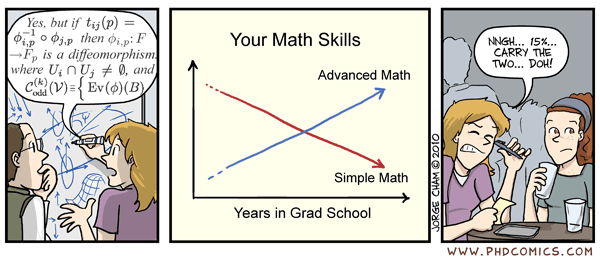
\includegraphics[width=0.8\textwidth]{pics/phd_comics.png}
\end{figure}
\newpage

\tableofcontents
\newpage

\setcounter{page}{1}
\pagestyle{fancy}
%советы для подопечных
\section*{Советы для семинаристов}
\addcontentsline{toc}{section}{Советы для семинаристов}

Часть этого руководства взята из плана к курсу Никиты Астраханцева (2017 год). Сами же советы были сформулированы Артемом Абановым. Были добавлены некоторые дополнения.
\begin{itemize}
    \item В начале каждого семинара делать наставления для школьников (2-3 минуты). Рассказать какую-нибудь байку или анекдот. 
    \item Школьники делятся на разные команды (столы) по их уровню знаний. Нужно сделать так, чтобы до школьника было близко идти, чтобы успеть поработать с каждым за вашим столом.
    \item Готовтесь к каждому семинару!!! Подумайте над задачами, которые вы можете дать конкретному школьнику, помимо заранее подготовленных. Сделайте это таким образом, чтобы вы их быстро могли вспомнить: сделайте распечатку, перепишите в тетрадь.
    \item Ваша задача - подобрать задачу уровня, немногим выше уровня школьника, чтобы ему/ей было комфортно, удобно и процесс был продуктивным.
    \item Если школьник решил задачу, то следует сделать следующее: 
    \begin{enumerate}
        \item Похвалить
        \item Проверить размерность/знак/ответ
        \item Обсудить предельные случаи. Поговорить о физике этих предельных случаев.
    \end{enumerate}
    \item Если задача у школьника вызывает затруднения, то стоит его подбодрить и помочь коротким советом.
    \item Если затруднения продолжаются, то стоит дать другую задачу, которая подведет к нерешенной задаче.
    \item Если видите, что школьники устали - рассказать байку/анекдот в тему занятия. 
    \item Всегда старайтесь добиться от школьника физического смысла, заложенного в формулах. Формулы - отражение физики задачи! 
\end{itemize}
\newpage
%первое занятие
\section{Функции одной переменной}
\epigraph{\textsf{Fear is the path to the dark side. Fear leads to anger, anger leads to hate, hate leads to suffering.}}{\texttt{Yoda}}
\paragraph{Зачем нам нужны функции?} Так исторически сложилось, что физические законы плохо интерпретируемы без использования какого-то вспомогательного аппарата/языка, который 
позволяет нам записывать эти законы. Функции - это один из таких языков, который позволяет нам записывать законы природы, а также решать задачи, которые возникают в физике. На первом занятии начнем с наиболее простых функций - функций одной переменной.
\subsection{Примеры функций}
\begin{definition}
    Функция $f$ от переменной $x$ - это правило, которое каждому значению $x$ сопоставляет значение $f(x)$.
\end{definition}
Каждому $x$ соотвествует какое-то значение $y = f(x)$, причем оно единственное. То есть если $x_1 = x_2$, то $f(x_1) = f(x_2)$.

\begin{prac}
   Постройте графики функции $f(x) = x$, $f(x) = x^2$, $f(x) = x^3$, $f(x) = \sqrt{x}$. Какой физический закон/формула/что угодно физическое интерпретируется этими зависимостями? 
\end{prac}
\subsection{Тригонометрические функции}
Допустим, у нас есть команда школьников, которая получала наряд по вычислению длины окружности радиуса $R$. Тогда для любого угла $\varphi$ мы можем определить положение школьников на окружности, которая соответствует этому углу. Эти координаты будут равны:
\begin{align*}
    x &= R \cos \varphi, \\
    y &= R \sin \varphi.
\end{align*}
Такие фукнции называются \textbf{тригонометрическими}. С помощью них можно охарактеризовать движение по окружности, колебания и много всего другого.

Понять что они из себя представляют довольно просто, если изобразить окружность единичного радиуса и провести луч, который образует угол $\varphi$ с положительным направлением оси $x$. Тогда координаты точки, в которой этот луч пересекает окружность, будут равны ($\cos \varphi$, $\sin \varphi$) (\texttt{см. на доску}). Отсюда сразу же следует \textbf{основное тригонометрическое тождество}:
\begin{equation*}
    \cos^2 \varphi + \sin^2 \varphi = 1.
\end{equation*}
\begin{prac}
    Постройте графики функции $f(x) = \sin x$, $f(x) = \cos x$, $f(x) = \tan x = \frac{\sin x}{\cos x}$. Укажите точки, где функции обращаются в ноль, где у них максимальное/минимальное значение, а также точки, где функции не определены. 
\end{prac}
\begin{rem}
    Тригонометрические функции периодичны, то есть для них выполняется $f(x + 2\pi) = f(x)$.
\end{rem}
Рассмотрим основные формулы приведения тригонометрических функций, которые вам пригодятся (наверняка):
\begin{eqnarray*}
    && \sin(\alpha + \beta) = \sin \alpha \cos \beta + \cos \alpha \sin \beta\\
    && \cos(\alpha + \beta) = \cos \alpha \cos \beta - \sin \alpha \sin \beta\\
\end{eqnarray*}

\begin{prac}
    Используя формулы приведения, получите:
    \begin{align*}
        \sin(2\alpha) &= 2 \sin \alpha \cos \alpha\\
        \cos(2\alpha) &= \cos^2 \alpha - \sin^2 \alpha = 2\cos^2 \alpha - 1 = 1 - 2\sin^2 \alpha\\
        \tan(2\alpha) &= \frac{2\tan \alpha}{1 - \tan^2 \alpha}\\
        \cos \alpha &= \sin (\frac{\pi}{2} - \alpha)
    \end{align*}
\end{prac}
\subsection{Показательная функция}
\begin{definition}
    Показательная функция - это функция вида $y = a^x$, где $a > 0$.
\end{definition}
Примерами таких функций могут служить $2^x, 5^x, (-1)^x$ и т.д. Если $a > 1$ - функция возрастает, если $a < 1$ - функция убывает. Возникает вопрос: как найти $x$, при котором $3^x = 4$?
\subsection{Логарифм}
Для этого вводится функция \textbf{логарифма}: $y = \log_a x$, которая является обратной к показательной функции. То есть $x = \log_a y$ - это такое число, что $a^x = y$.
Эта функция определена при $a > 0$, $a \neq 1$, и ее область определения - все положительные $x$. 
\begin{prac}
    Нарисовать графики функции $y = \log_a x$ при $a > 1, a < 1$.
\end{prac}
Наиболее простым и популярным основанием для этой функции является число $e \approx 2.71828$, которое называется \textbf{числом Эйлера}. Тогда функция $\log_e x$ обозначается как $\ln x$ и называется \textbf{натуральным логарифмом}. 
Число $e$ мы поподробнее обсудим на следующей \texttt{Ушке}.

\begin{remark}
    Принято не работать с логарифмами, основания у которых отличны от $e$. В таком случае использует свойства логарифма $\log_a x = \frac{\ln x}{\ln a}$.
\end{remark}

\newpage
\renewcommand{\thesubsection}{\roman{subsection}}
\setcounter{subsection}{0}
\markboth{Задачи}{Задачи}
\addcontentsline{toc}{section}{Задачи}
\section*{Задачи}


\newpage
\markboth{Контрольная работа}{Контрольная работа}
\addcontentsline{toc}{section}{Контрольная работа}
\section*{Контрольная работа}
% \input{tasks/exam.tex}

\end{document}
